\documentclass{beamer}
\usepackage[utf8]{inputenc}
% \usepackage{polski}
% \usepackage[polish]{babel}
\usepackage[T1]{fontenc}
\usepackage{tikz}
\usepackage{tikzducks}
% \usetikzlibrary{decorations.pathmorphing}
\usepackage{multimedia}
\usepackage{graphicx}
\usepackage[justification=centering]{caption}
\usepackage{textcomp}
\usepackage{appendixnumberbeamer}
\usepackage{qrcode}
\usepackage[natbib, sorting=none, maxbibnames=99]{biblatex}
\addbibresource{lio.bib}
\usepackage{hyperref}
%\usepackage[width=\textwidth]{animate}
%\usepackage{chemformula}
\usepackage{sidecap}
\usepackage{multirow}
\usepackage{rotating}
\usepackage{anyfontsize} % change font size for semposiwko
\usepackage{subcaption}


% \usepackage[natbib, language=polish, sorting=none]{biblatex}
% \addbibresource{lio.bib}
\renewcommand*{\bibfont}{\scriptsize}

\usetheme{Szeged}
\usecolortheme{whale}
\setbeamercolor{palette primary}{bg=violet!80!black,fg=white}
\setbeamercolor{palette secondary}{bg=violet!60!black,fg=white}
\setbeamercolor{palette tertiary}{bg=violet!40!black,fg=white}
\setbeamercolor{palette quaternary}{bg=violet!20!black,fg=white}
\setbeamercolor{structure}{fg=violet!60!black}
\setbeamertemplate{caption}{\insertcaption}
% \setbeamertemplate{headline}{
%   \begin{beamercolorbox}[wd=.9\paperwidth]{headline}
%     \vspace{1.5ex}
%     \insertsectionnavigationhorizontal
%     \vspace{1.5ex}
%   \end{beamercolorbox}
% }

\linespread{0.6}

\setbeamertemplate{background}%
{%
    \begin{tikzpicture}[remember picture,overlay]{\node[yshift=1.5cm,xshift=-2cm,opacity=0.1] at (current page.south east)
      {
      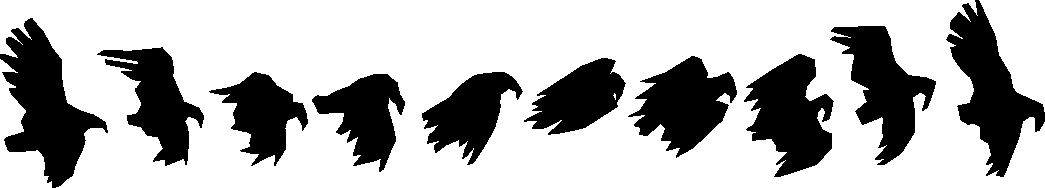
\includegraphics[scale=0.4, angle=20]{ptaki.pdf}
      }
      ;
    \node[yshift=1.0cm,xshift=0.6cm] (logopos) at (current page.south west) {{\begin{tikzpicture}\shuffleducks\duck[signpost=\insertframenumber, \randomhead,scale=.4]\end{tikzpicture}}};
    \pgfmathsetmacro{\progress}{360*(\insertframenumber)/(\inserttotalframenumber)};
    \draw[line width=0.2*3pt] ([xshift=0.55cm] logopos)  arc[radius=0.55cm, start angle=0, end angle=\progress];
    \fill ([shift={(\progress:0.55cm)}] logopos) circle(1pt);

    }
        \end{tikzpicture}
    
}

\newcommand{\SeMPowisko}{%
\large S\normalsize%
\kern-.3em \lower.2ex\hbox{e}%
\lower.2ex\hbox{\large M\normalsize}%
\kern-.1em \raise.1ex\hbox{\large P\normalsize}%
\kern-.3em \lower.2ex\hbox{o}%
\kern-.2em \raise.2ex\hbox{w}%
\lower.2ex\hbox{i}%
s%
\raise.2ex\hbox{k}%
\kern-.3em \lower.2ex\hbox{o}%
}



\title{Hierarchical autoregressive neural networks in three-dimensional statistical system}
% \subtitle{Przegląd niektórych eksperymentów}
\author[M. Winiarski]{Mateusz "$\blacksquare$" Winiarski\\{\tiny under supervision of dr Tomasz Stebel}}
\institute[WFAIS UJ]{experimental physics$^\dagger$, WFAIS UJ}
\date[today]{May 8th, 2025}

\begin{document}

\frame{\titlepage}

\nocite{*}

\section{Neural networks}
\begin{frame}{Neural network: what you think it is}
\begin{columns}
\begin{column}{0.5\textwidth}
    \begin{figure}
        \centering
        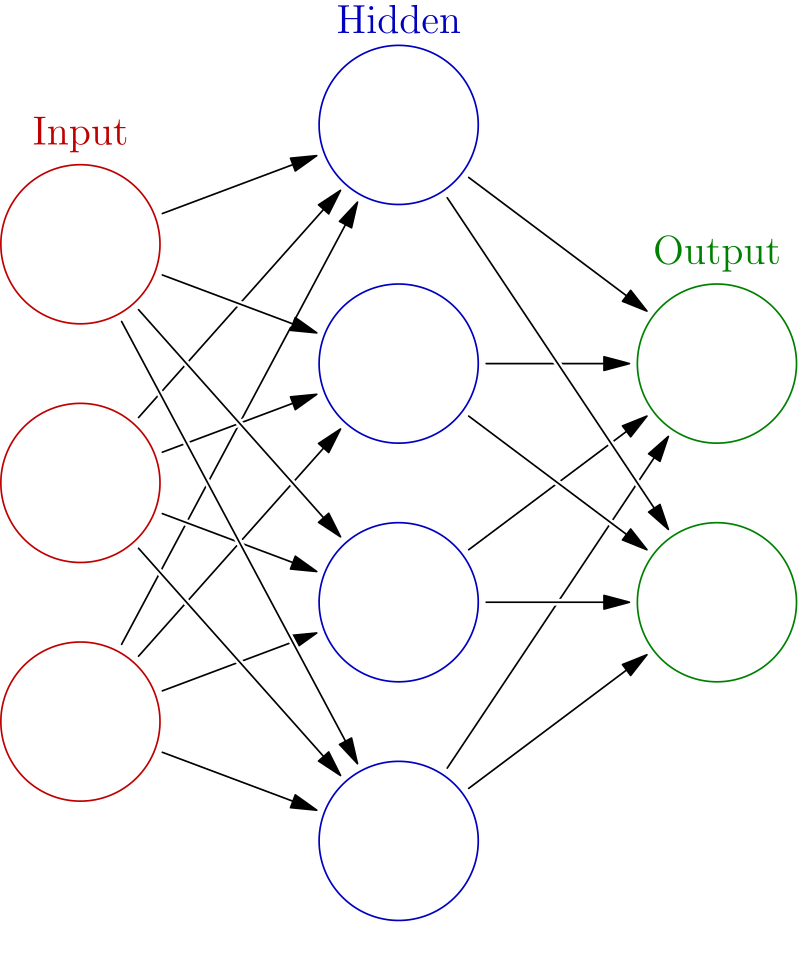
\includegraphics[width=0.7\linewidth]{neural.png}
        \caption{First Google Image search result for string \texttt{"neural network"}}
    \end{figure}
    \pause
    \end{column}
\begin{column}{0.5\textwidth}
    \begin{figure}
        \centering
        
\includegraphics[width=0.9\linewidth]{tumblr_eca910e5002963c22463127d53d496e4_ed0409bc_1280.jpg}
        \caption{Your reaction to that information}
    \end{figure}
\end{column}
\end{columns}
\end{frame}

\begin{frame}{Neural network: what it really is}
    \begin{figure}
        \centering
        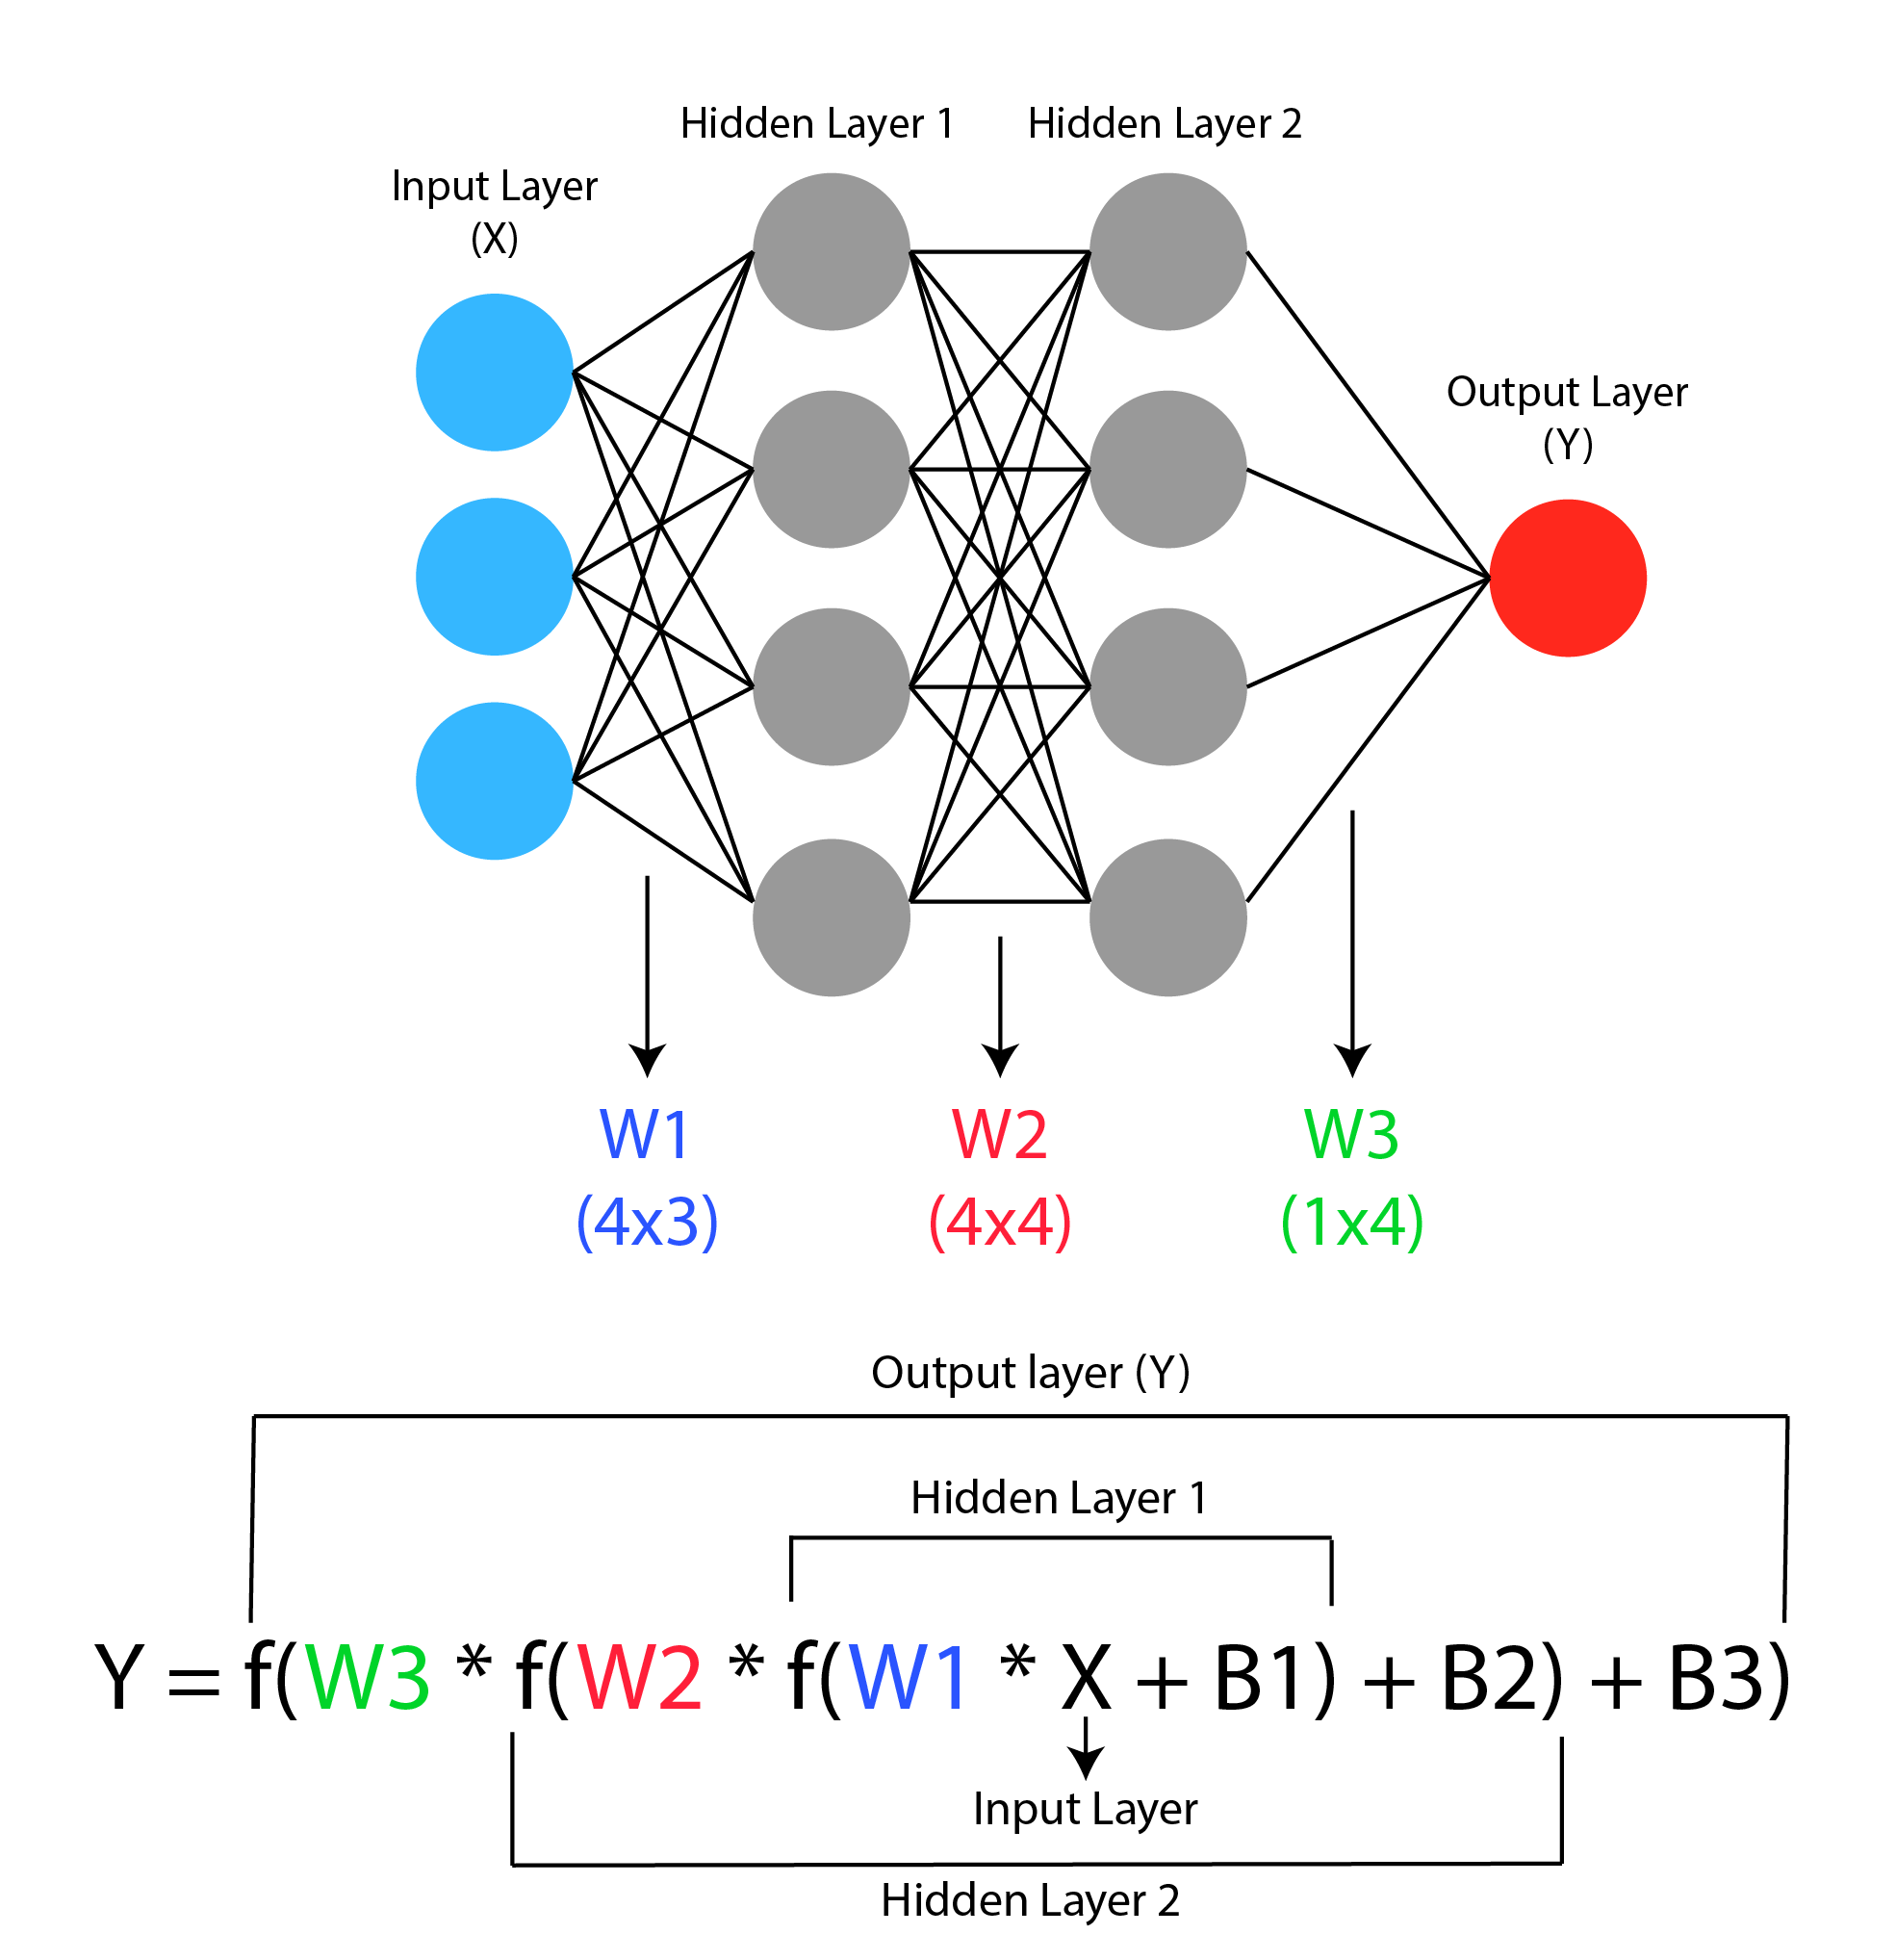
\includegraphics[width=0.55\textwidth]{reality.png}
        \caption{In physics, everything is a matrix}
    \end{figure}
\end{frame}

% \begin{frame}{Neural network: what it does}
% \vspace{-1.5cm}
%     \begin{columns}
%         \begin{column}{0.35\textwidth}
%             \begin{figure}
%                 \centering
%                 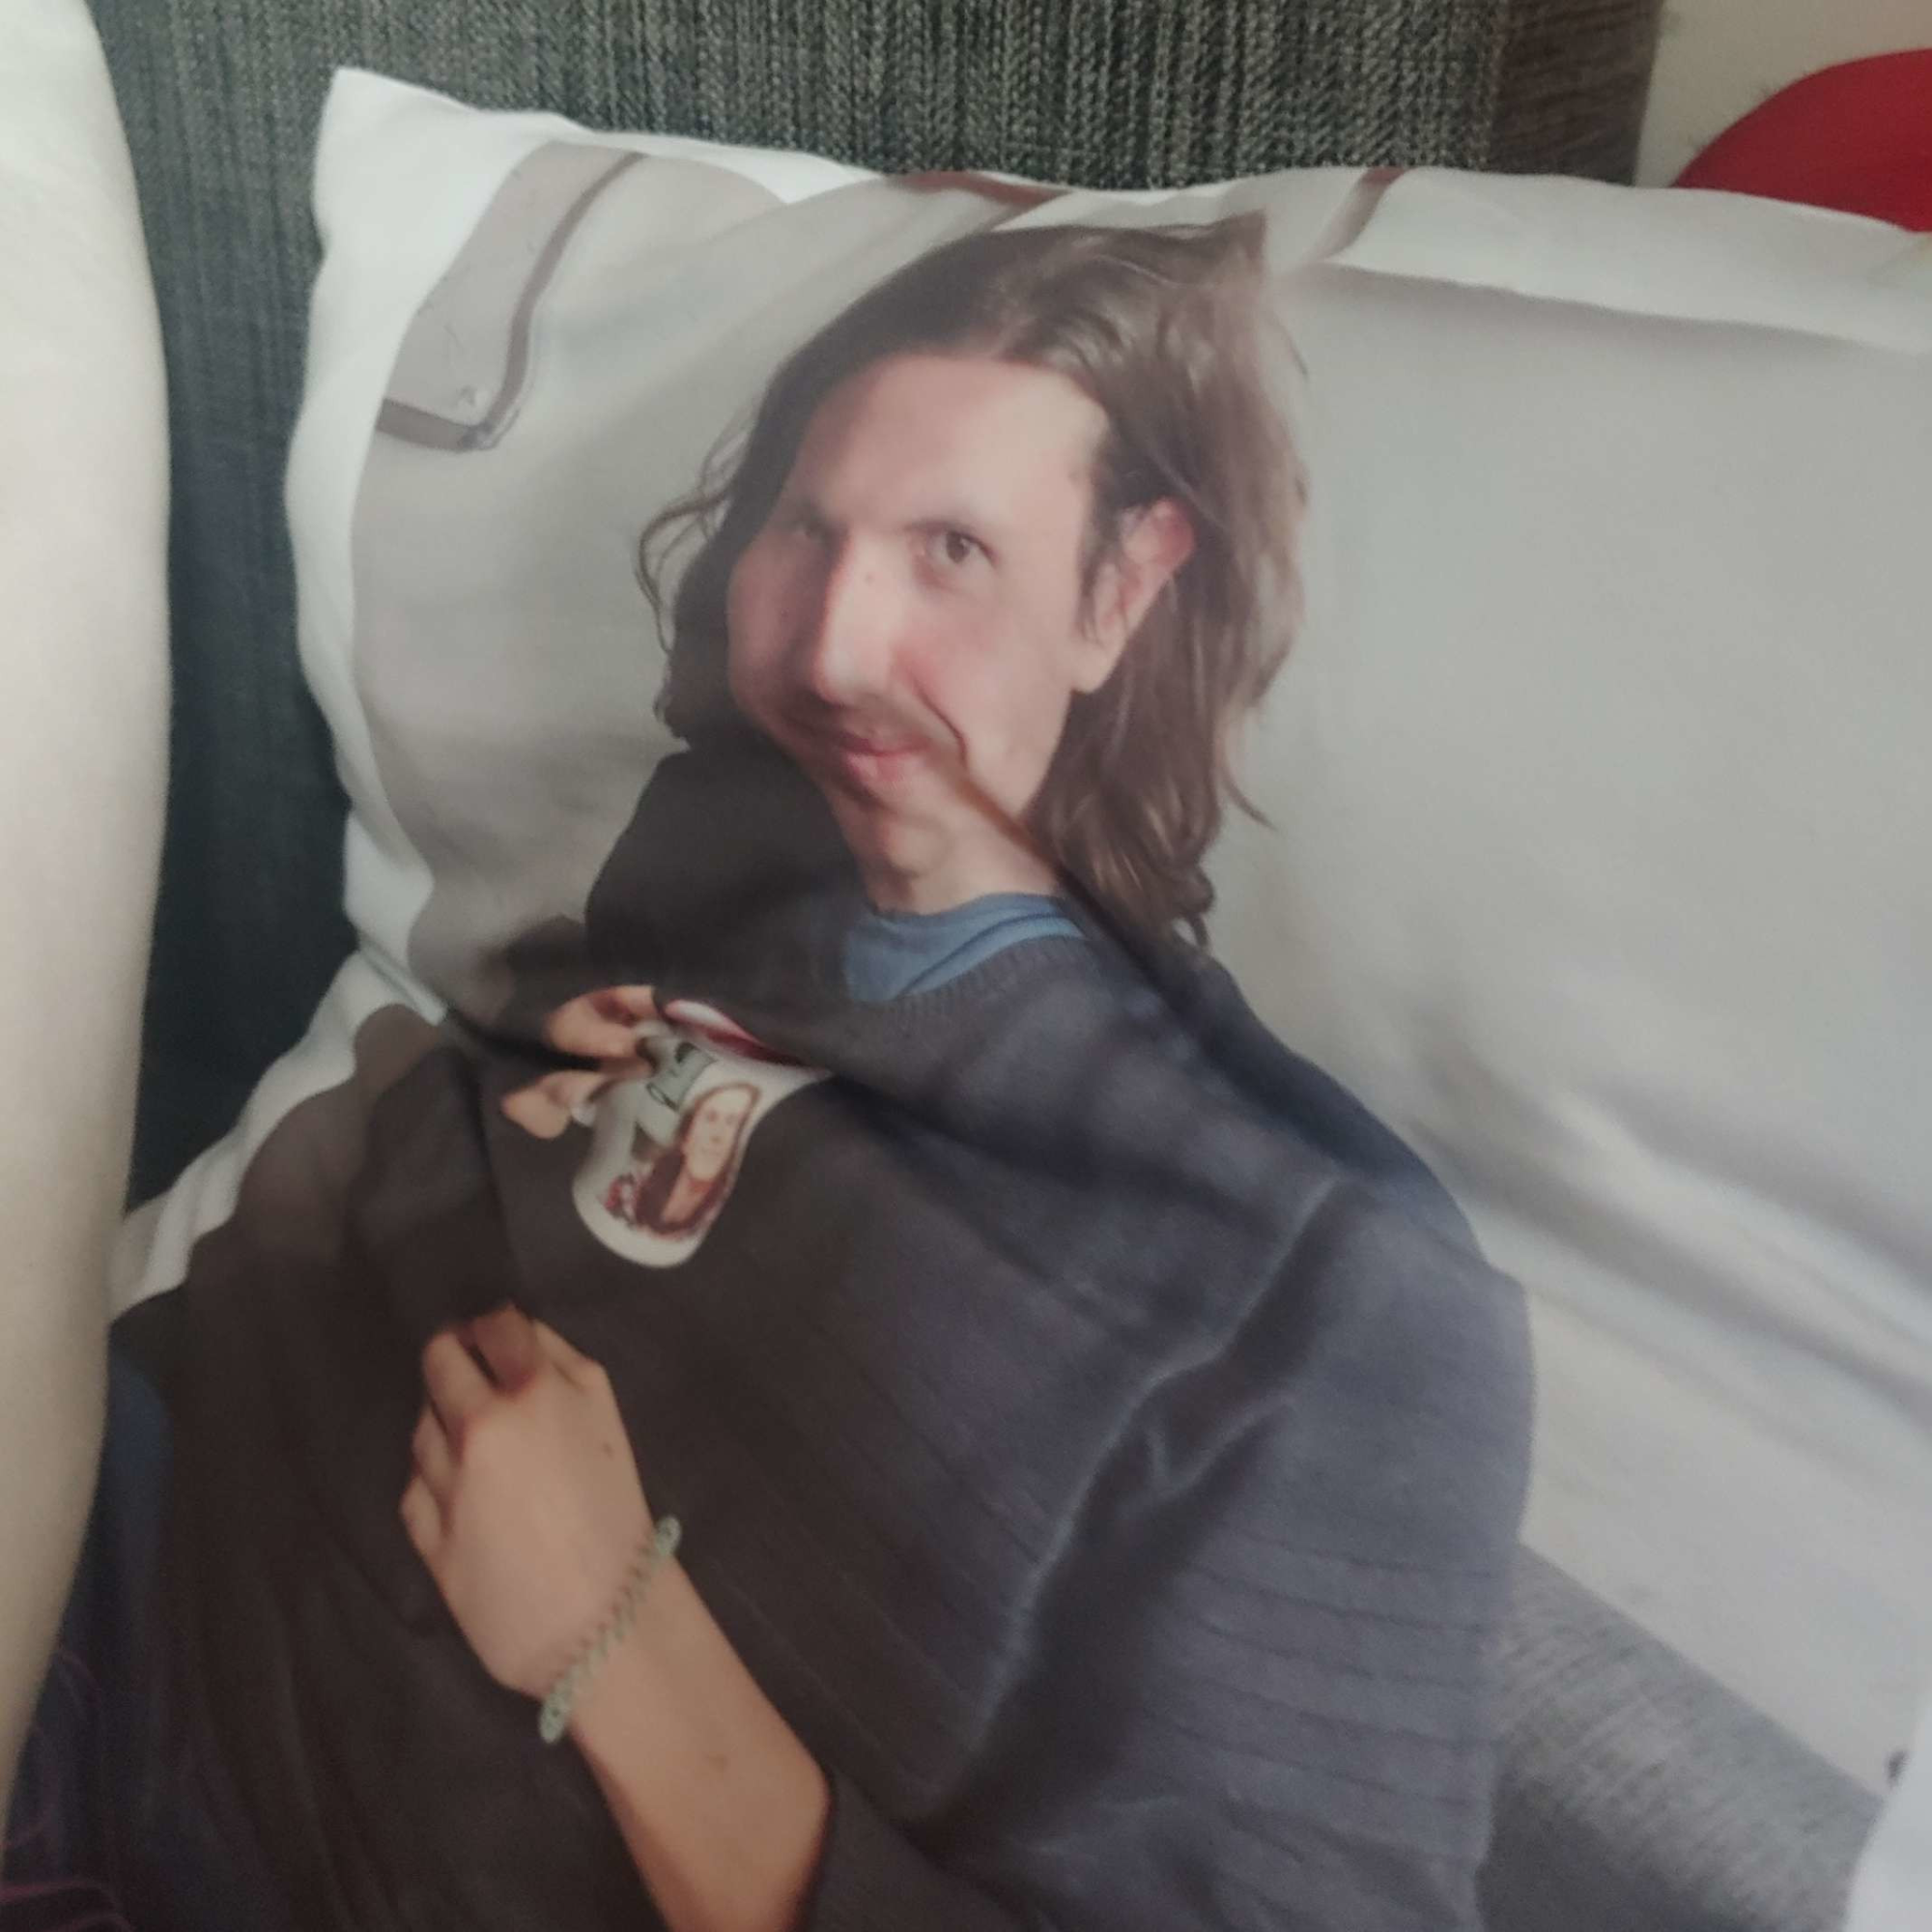
\includegraphics[width=\linewidth]{distorted/distorted.png}
%             \end{figure}\pause
%         \end{column}
%         \begin{column}{0.05\textwidth}
%             \begin{figure}
%                 \centering
%                 
\includegraphics[width=\linewidth]{distorted/distorted-0-0}
%                 
\includegraphics[width=\linewidth]{distorted/distorted-0-1}
%                 
\includegraphics[width=\linewidth]{distorted/distorted-0-2}
%                 
\includegraphics[width=\linewidth]{distorted/distorted-0-3}
%                 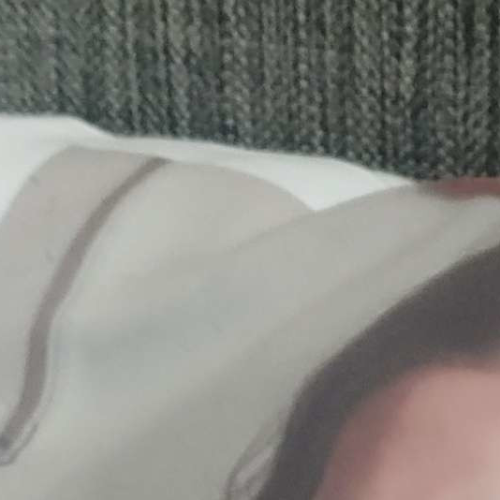
\includegraphics[width=\linewidth]{distorted/distorted-1-0}
%                 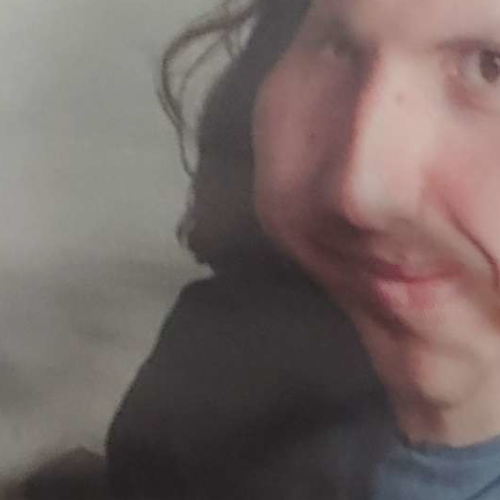
\includegraphics[width=\linewidth]{distorted/distorted-1-1}
%                 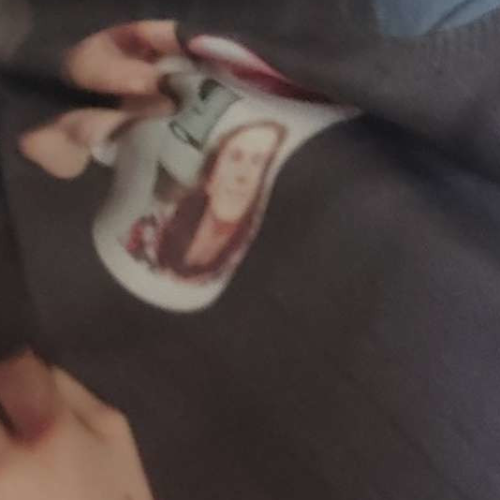
\includegraphics[width=\linewidth]{distorted/distorted-1-2}
%                 
\includegraphics[width=\linewidth]{distorted/distorted-1-3}
%                 
\includegraphics[width=\linewidth]{distorted/distorted-2-0}
%                 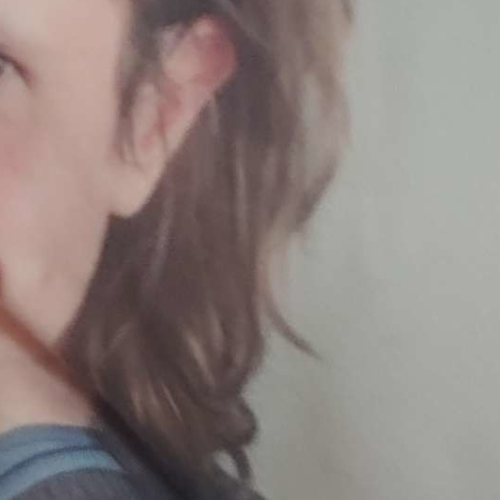
\includegraphics[width=\linewidth]{distorted/distorted-2-1}
%                 
\includegraphics[width=\linewidth]{distorted/distorted-2-2}
%                 
\includegraphics[width=\linewidth]{distorted/distorted-2-3}
%                 
\includegraphics[width=\linewidth]{distorted/distorted-3-0}
%                 
\includegraphics[width=\linewidth]{distorted/distorted-3-1}
%                 
\includegraphics[width=\linewidth]{distorted/distorted-3-2}
%                 
\includegraphics[width=\linewidth]{distorted/distorted-3-3}
%             \end{figure}\pause
%         \end{column}
%         \begin{column}{0.3\textwidth}
%             \begin{figure}
%                 \centering
%                 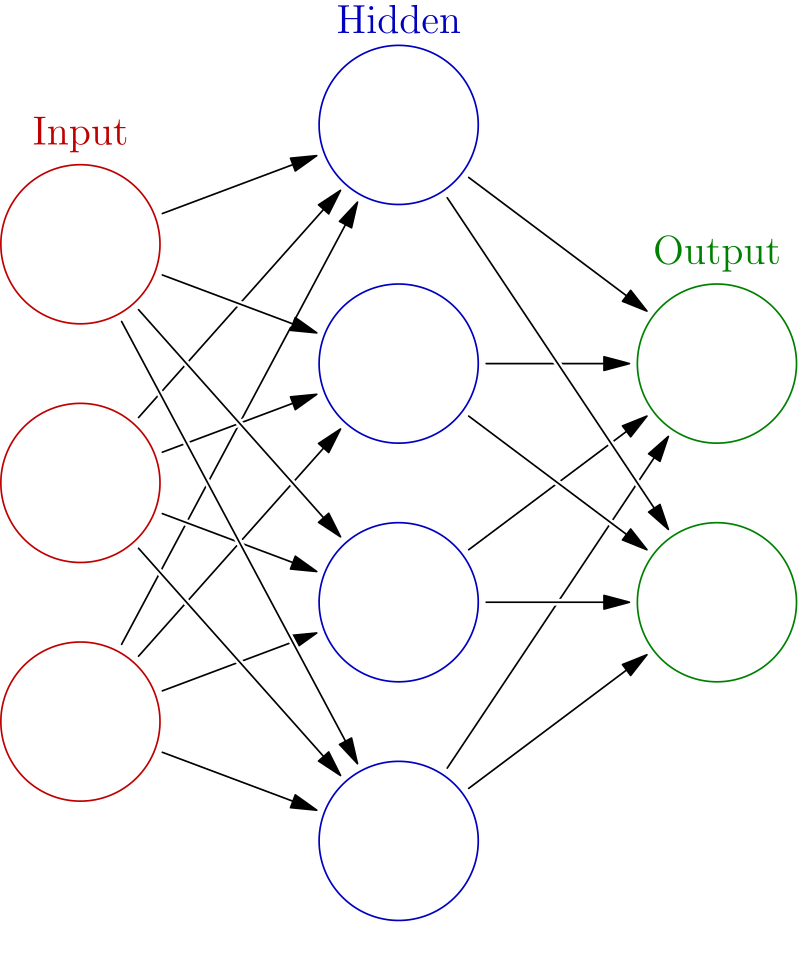
\includegraphics[width=\linewidth]{neural.png}
%             \end{figure}\pause
%         \end{column}
%         \begin{column}{0.2\textwidth}
%             \begin{tabular}{ll}
%                 Firlej & 0.95 \\
%                 cushion & 0.82 \\
%                 mug & 0.53 \\
%                 hair & 0.42 \\
%                 hand & 0.34
%             \end{tabular}
%         \end{column}
%     \end{columns}
% \end{frame}


\subsection{Autoregressive neural networks}

\begin{frame}{Autoregression}
    $$X_t = \sum_{i=1}^p \varphi_i X_{t-i} + \varepsilon_t$$
    \begin{figure}
        \centering
        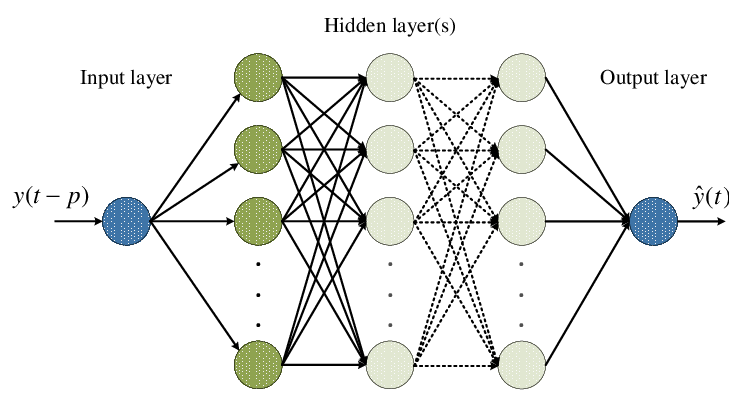
\includegraphics[width=0.8\textwidth]{ann.png}
        \caption{An example of autoregressive neural network (source: \cite{balanici2019})}
    \end{figure}
    
\end{frame}

\subsection{Hierarchical neural networks}

\begin{frame}{Hierarchy}
    \begin{figure}
        \centering
        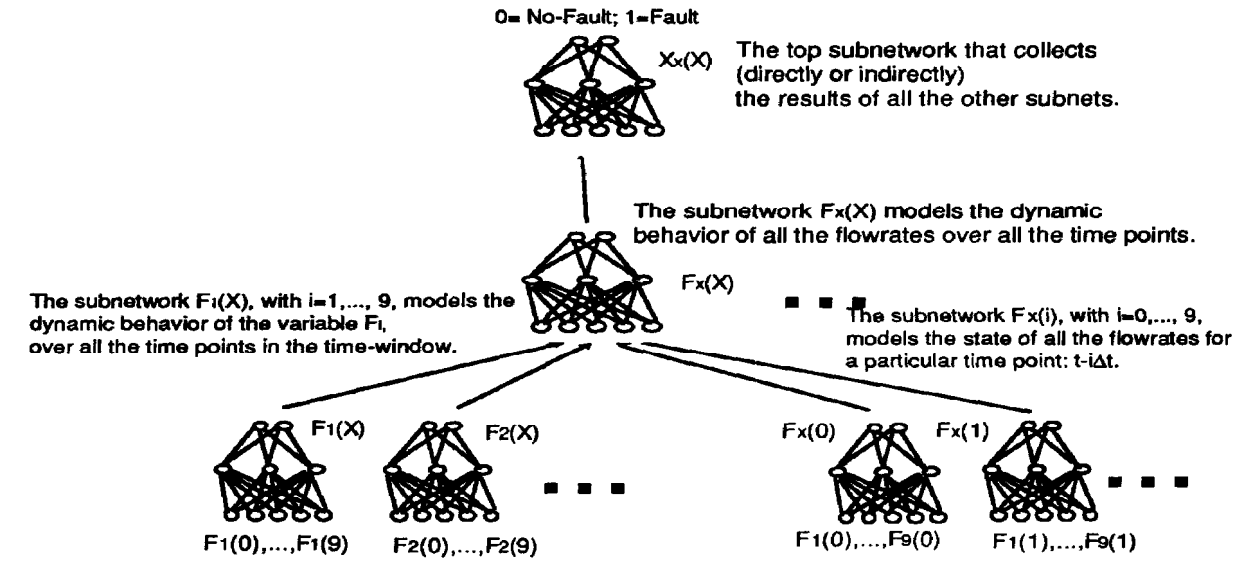
\includegraphics[width=0.9\textwidth]{hier.png}
        \caption{An example of hierarchical neural network (source: \cite{mavrovouniotis1992hierarchical})}
    \end{figure}
\end{frame}

\section{HANs in statistical physics}

\subsection{Ising model}
\begin{frame}{What is spin}
    \begin{figure}
        \centering
        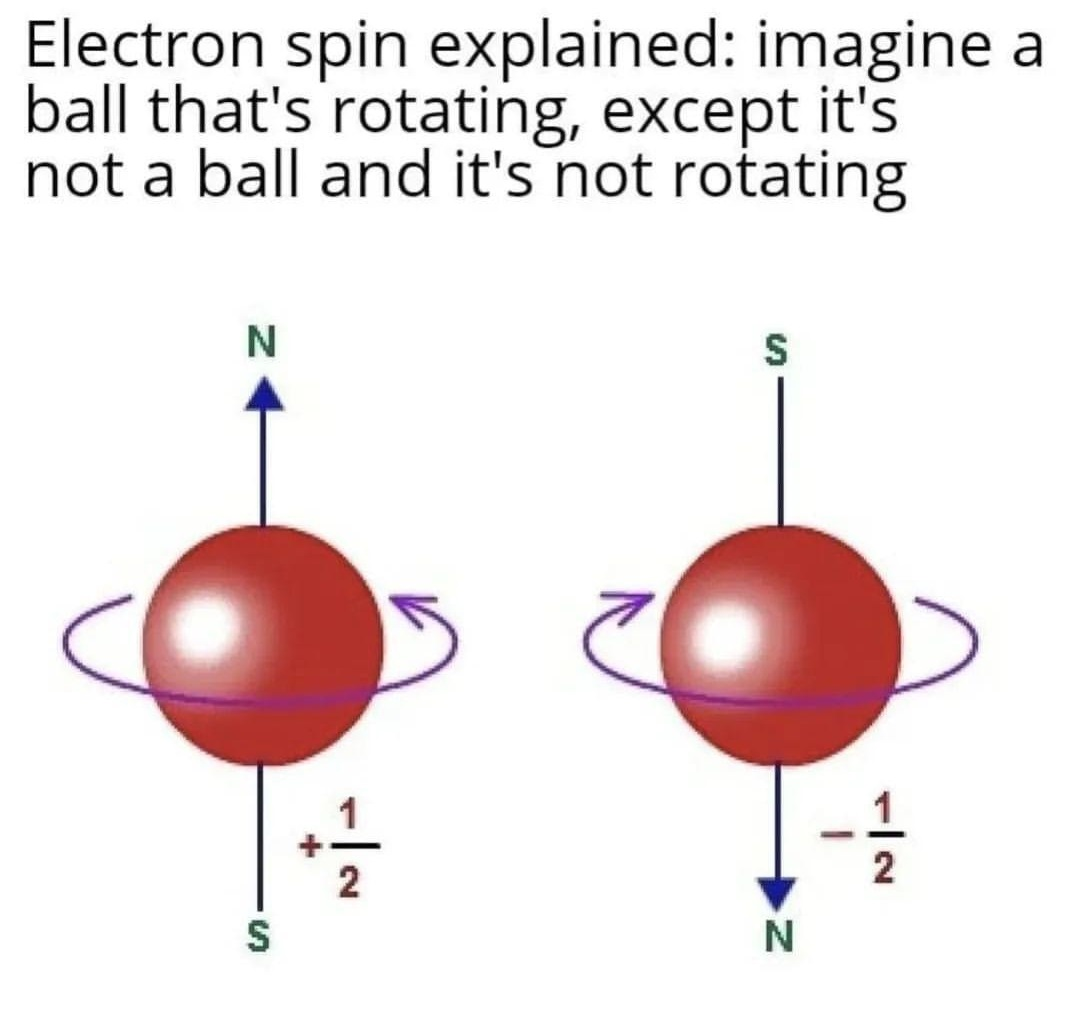
\includegraphics[width=0.5\textwidth]{spin.jpg}\pause
        \caption{This is not what spin means}
    \end{figure}
\end{frame}

\begin{frame}{What is spin, again}
    \begin{figure}
        \centering
        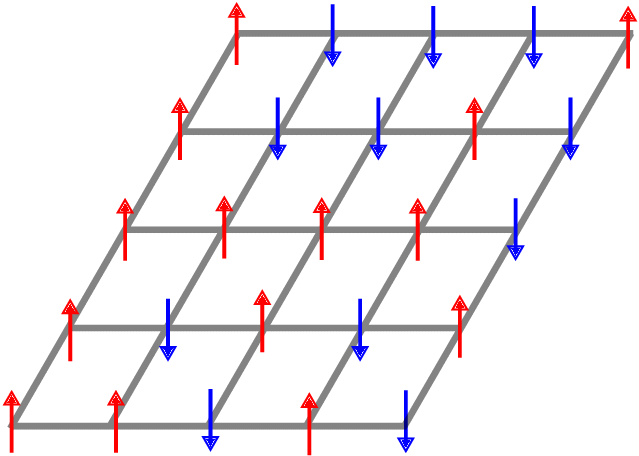
\includegraphics[width=0.8\textwidth]{ising.png}
        \caption{Illustration of 2D Ising model}
    \end{figure}
\end{frame}

\begin{frame}{Some physics now: Ising model}
    \begin{itemize}
        \item $\sigma$ -- configuration  (microstate)
        \item assumption: no external magnetic field
    \end{itemize}
    \begin{columns}
        \column{0.5\textwidth}
    $$M(\sigma)=\sum_{i\in\text{spins}} s_i$$
    $$E(\sigma)=-\frac{1}{2}\sum_{i,j\in\text{neighbours}} s_i s_j$$
    $$p(\sigma)=\frac{e^{-\beta E(\sigma)}}{Z}$$
    $$Z=\sum_\sigma e^{\beta E(\sigma)}$$
        \column{0.5\textwidth}
        $$F=-\frac{1}{\beta}\log Z$$
        $$S=\beta(U-F)$$
        $$\beta=\frac{1}{k_B T}$$
    \end{columns}
\end{frame}

\begin{frame}{Limitations of MCMC algorithms}
    (\emph{MCMC} -- Monte Carlo Markov chain)
    \vfill
    Limitations:
    \begin{itemize}
        \item no access to partition function $Z$ $\to$ can't compute $F$ and $S$
        \item critical slowing down near phase transitions (at $\beta_c)$
        \item exponential scaling in 3D systems for brute-force methods
    \end{itemize}
\end{frame}

\begin{frame}{How to apply hierarchy}
    \begin{columns}
        \column{0.4\textwidth}
    \begin{figure}
        \centering
        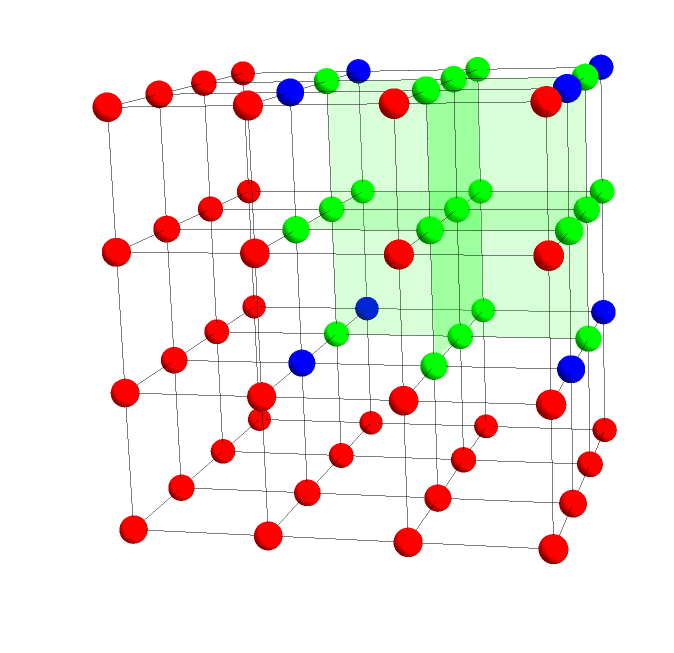
\includegraphics[width=0.8\linewidth]{hierarchy.png}
        \caption{Hierarchy in 4x4x4 cube}
    \end{figure}
        \column{0.6\textwidth}
    \begin{figure}
        \centering
        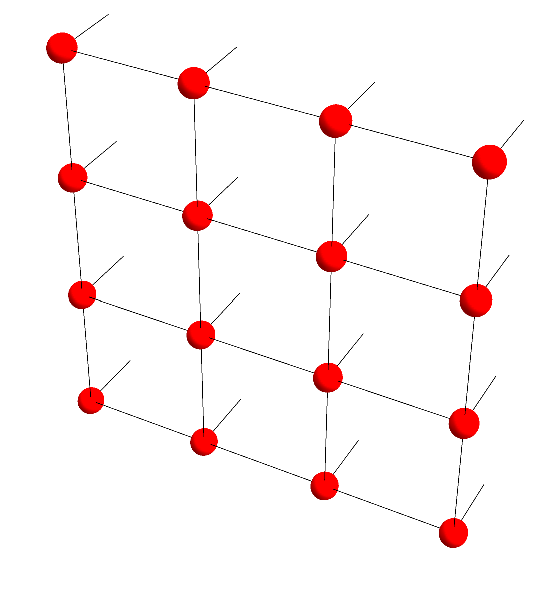
\includegraphics[width=0.22\linewidth]{plots/slice1.pdf}
        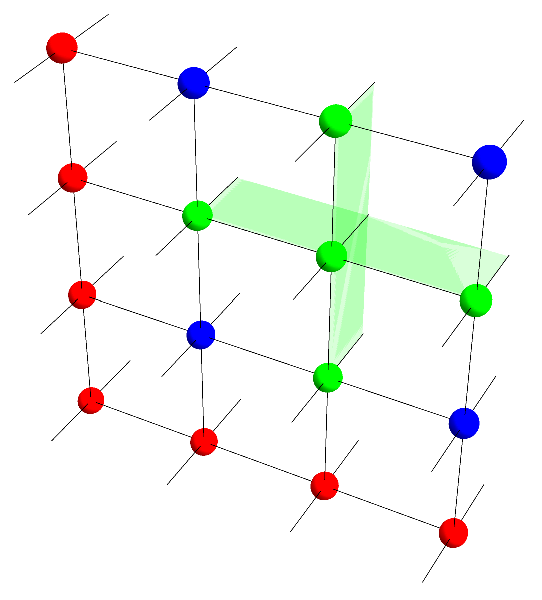
\includegraphics[width=0.22\linewidth]{plots/slice2.pdf}
        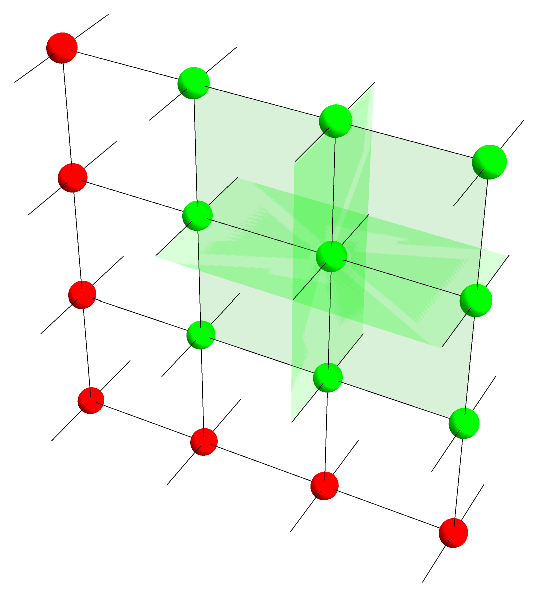
\includegraphics[width=0.22\linewidth]{plots/slice3.pdf}
        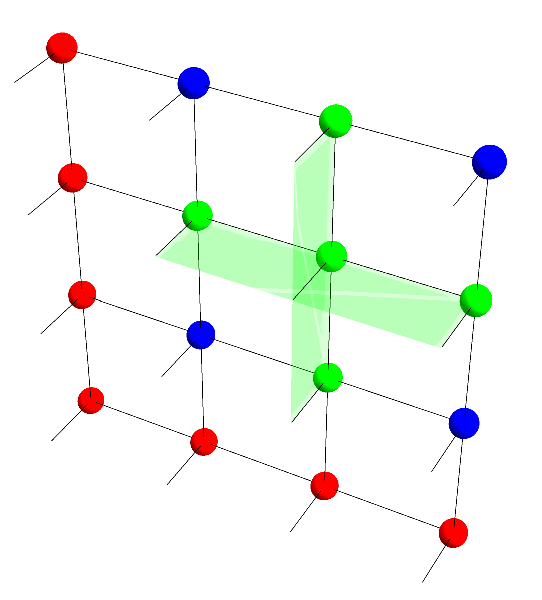
\includegraphics[width=0.22\linewidth]{plots/slice4.pdf}
        \caption{Slices of the left figure}
    \end{figure}
    \begin{align*}p(\mathbf{s}) &= p(\textrm{B}(\mathbf{s})) p(\textrm{I}(\mathbf{s})| \textrm{B}(\mathbf{s})) \\ &= p(\textrm{B}(\mathbf{s})) \prod_{a=1}^{6} p(\textrm{I}^a(\mathbf{s})| \textrm{B}^a(\mathbf{s})).
        \end{align*}
    \end{columns}
\end{frame}

\begin{frame}{How to apply autoregression}
    $$F=-\frac{1}{\beta} \log Z$$
    $$F=\frac{1}{\beta} \sum_{i\in\text{configurations}} q_\theta(\sigma_i)[\beta E(\sigma_i)+\log q_\theta(\sigma_i)]$$
\end{frame}

\begin{frame}{Algorithm workflow}
\begin{columns}
\column{0.7\textwidth}
\text{step 1: hierarchical training}
\begin{itemize}
    \item \textcolor{red}{level 1}: boundary spins (2D-like network)
    \item \textcolor{green}{level 2}: cross-structure (smaller network)
    \item \textcolor{blue}{level 3}: isolated spins (heatbath)
\end{itemize}
\column{0.3\textwidth}

    \begin{figure}
        \centering
        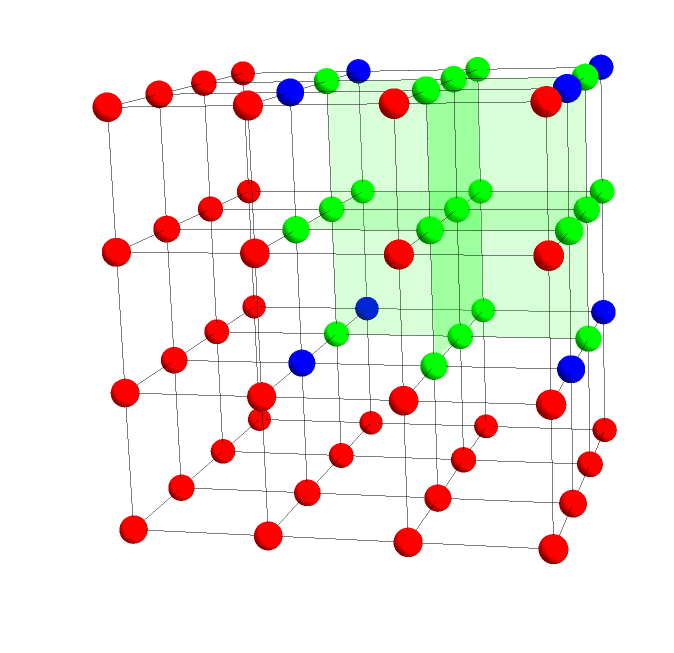
\includegraphics[width=0.8\linewidth]{hierarchy.png}
    \end{figure}
\end{columns}

\text{step 2: autoregressive sampling}
\begin{equation*}
q_\theta(\mathbf{s}) = \prod_{i=1}^N q_\theta(s^i | s^{1},\ldots,s^{i-1})
\end{equation*}

\text{step 3: Neural Importance Sampling \emph{(NIS)}}
\begin{equation*}
\langle O \rangle = \frac{1}{N\hat{Z}}\sum_i \hat{v}(\mathbf{s}_i)O(\mathbf{s}_i)
\end{equation*}
\end{frame}


\section{Results}

\subsection{Some plots}
\begin{frame}{Magnetization: Monte Carlo vs neural network}
\begin{figure}
    \centering
    \begin{subfigure}{0.45\textwidth}
    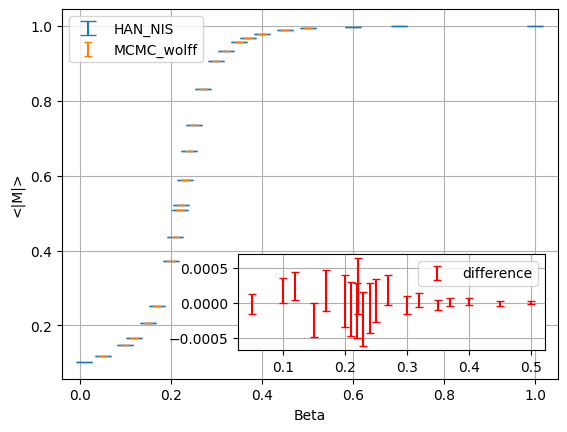
\includegraphics[width=\textwidth]{plots/m4.png}
    \caption{4x4x4}
    \end{subfigure} 
    \hfill
    \begin{subfigure}{0.45\textwidth}
    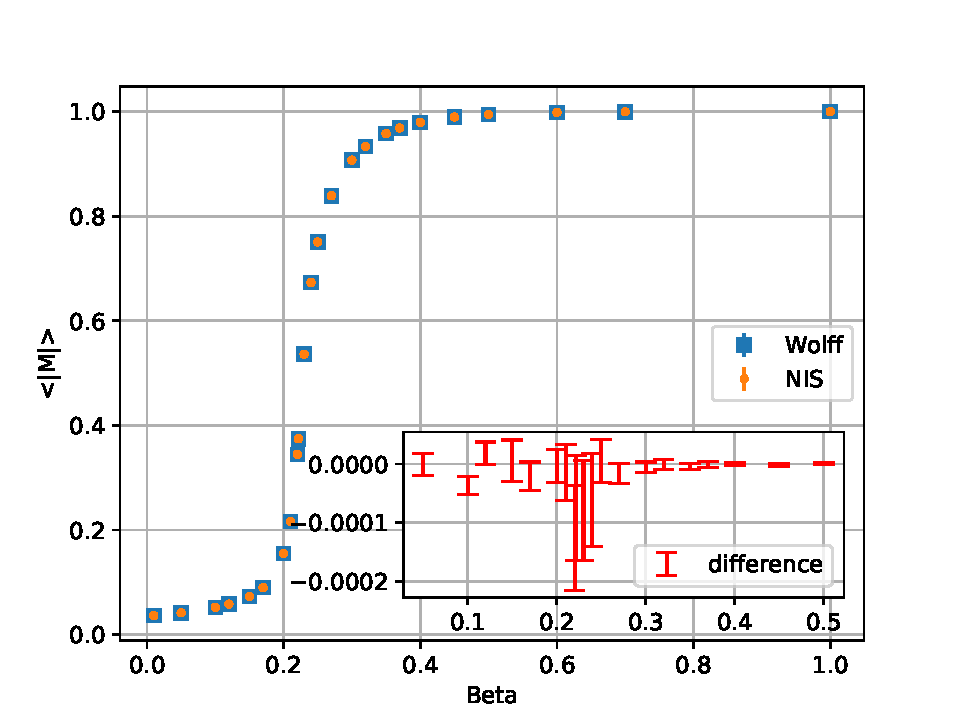
\includegraphics[width=\textwidth]{plots/m8.pdf}
    \caption{8x8x8}
    \end{subfigure}
    \caption{Magnetization vs temperature function $\beta$}
\end{figure}
\end{frame}

\begin{frame}{Extensive properties: neural network}
\begin{figure}
    \centering
    \begin{subfigure}{0.45\textwidth}
    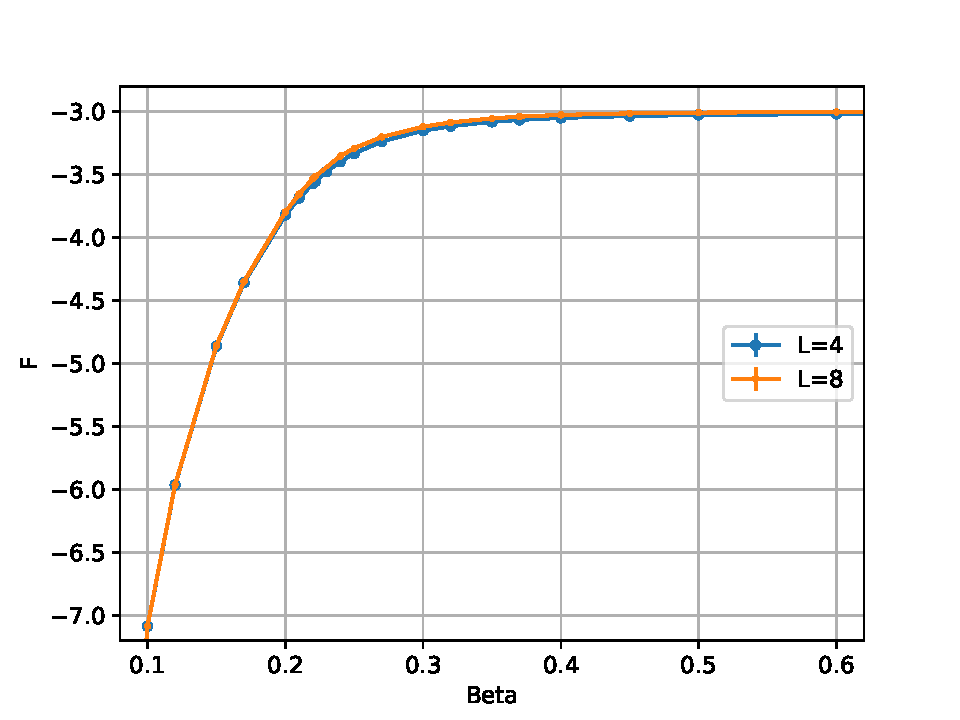
\includegraphics[width=\textwidth]{plots/f.pdf}
    \caption{free energy}
    \end{subfigure} 
    \hfill
    \begin{subfigure}{0.45\textwidth}
    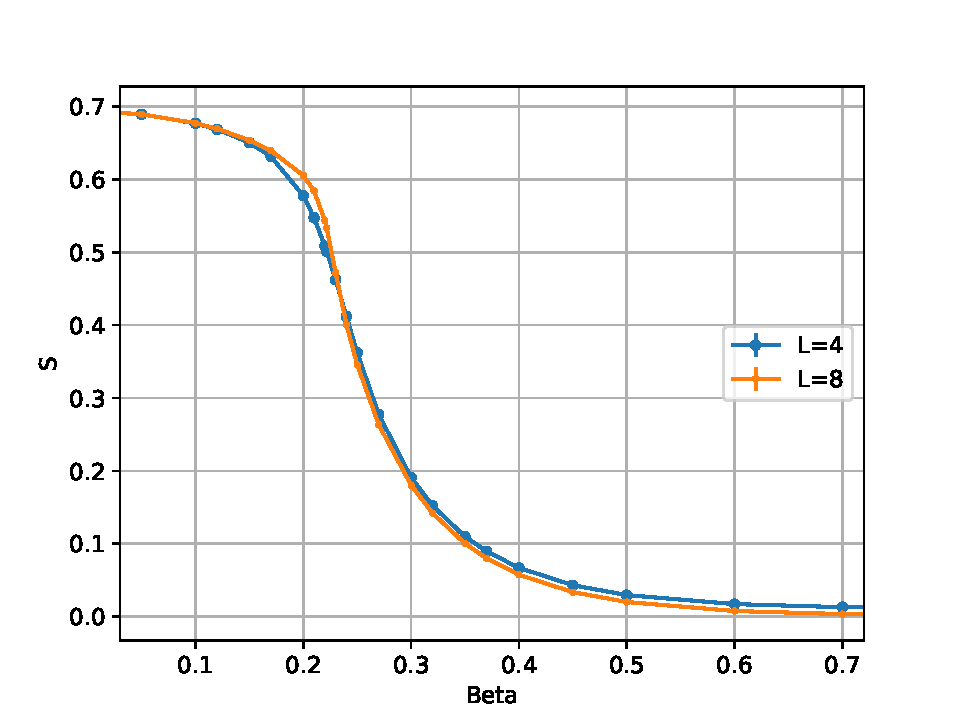
\includegraphics[width=\textwidth]{plots/s.pdf}
    \caption{entropy}
    \end{subfigure}
    \caption{Extensive parameters vs temperature parameter $\beta$ for 4x4x4 and 8x8x8 nets}
\end{figure}
\end{frame}

\subsection{Numerical results}

\begin{frame}{Timing}{}

        \begin{figure}
        \centering
        \begin{columns}
            \column{0.6\textwidth}
        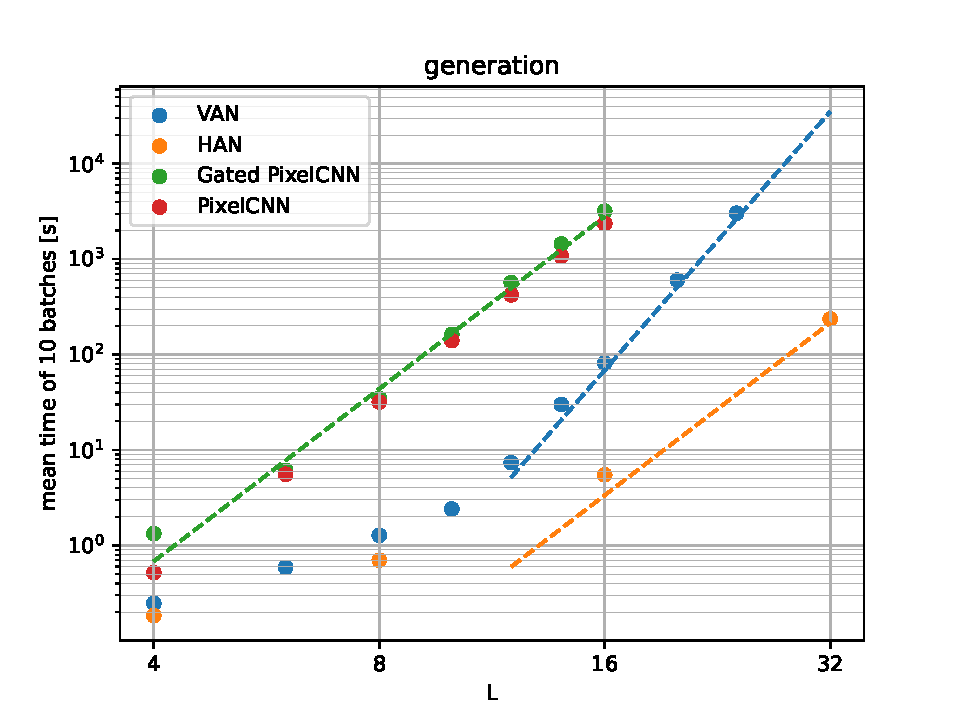
\includegraphics[width=1\linewidth]{plots/speedge.pdf}

            \column{0.4\textwidth} \small
        \caption{Mean time (in seconds) of 10 batches generation of VAN (blue circles), HAN (orange circles), PixelCNN (red circles) and Gated PixelCNN (green circles) algorithms in dependence on system linear size~$L$. Asymptotic approximations $\alpha L^9$ (blue dashed line), $\beta L^6$ (orange
dashed line) and $\gamma L^6$ (green dashed line), for VAN, HAN and Gated PixelCNN accordingly, were superposed on plots}
        \end{columns}
    \end{figure}
\end{frame}

        \newcommand{\avg}[1]{\left\langle{#1}\right\rangle}
\begin{frame}{Timing: 2D vs 3D}
        \begin{figure}
            \begin{columns}
                \column{0.7\textwidth}
        \centering
        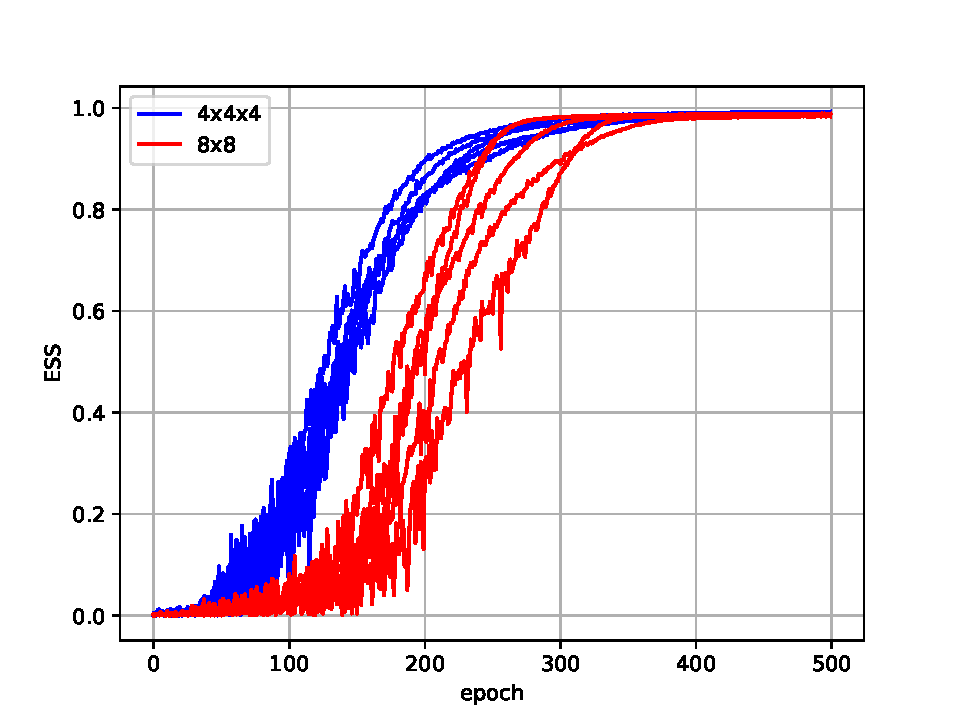
\includegraphics[width=\linewidth]{plots/ess_0.005.pdf}
        \column{0.3\textwidth}
        $ESS$ -- effective sample size
        \begin{align*}
    ESS &= \frac{\avg{\hat{w}}_{q_\theta}^2}{\avg{\hat{w}^2}_{q_\theta}} \\
    &\approx \frac{\left(\sum_{i=1}^N \hat w(\mathbf{s}_i)\right)^2}{N \sum_{i=1}^N \hat w^2(\mathbf{s}_i)}
% \label{ESS_definition}
\end{align*}
\end{columns}
        \caption{Comparison of the ESS growth for 4x4x4 (blue) and 8x8 (red) systems in a corresponding critical temperature $\beta$ (0.22 for the 3D and 0.38 for the 2D system)}
    \end{figure}
\end{frame}

\begin{frame}{Timing: comparison to classical algorithms}{}
    parameters: $10^9$ configurations, magnetization error $2\cdot 10^-6$
    \begin{itemize}
        \item HAN: 430 s for training + 3400 s for generation
        \item Wolff algorithm: 47 s
    \end{itemize}
\end{frame}



\section*{~}

\begin{frame}{Bibliography}{}
    {\footnotesize
    % \begin{thebibliography}{7}
        
    % \bibitem{hierarchical}Hierarchical autoregressive neural networks for statistical systems, \texttt{arXiv:2203.10989}
    % \bibitem{solving}Solving Statistical Mechanics Using Variational Autoregressive Networks, \texttt{arXiv:1809.10606}
    % \bibitem{thermalisation} Thermalisation and Relaxation of Quantum Systems, \texttt{doi:10.13140/RG.2.2.25169.63842}
    % \bibitem{hierarchical} Hierarchical neural networks, \texttt{doi:10.1016/0098-1354(92)80053-C}
    % \end{thebibliography}
    \nocite{*}
    \printbibliography[heading=none]}
\end{frame}

\begin{frame}{}

\begin{figure}

\centering
    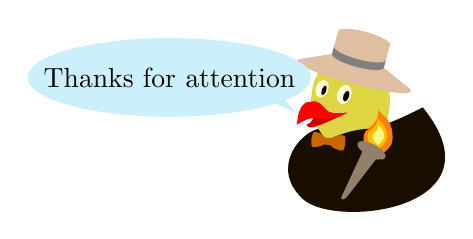
\begin{tikzpicture}
      \duck[parrot, body=gray!30!yellow, head=gray!30!yellow, bill=red, torch=gray!70!brown, tshirt=orange!10!black, strawhat=brown!50!white, ribbon=gray, bowtie=orange!80!black]
      %\addwater{blue!50!cyan}
      \fill[cyan!20!white] (-1.4,1.8) ellipse (1.8 and 0.5);
  \fill[cyan!20!white] (-0.2,1.54) -- (0.2,1.35) -- (0.0,1.6) -- cycle;
	\node at (-1.4,1.8) {Thanks for attention};
    \end{tikzpicture}
    \end{figure}


    
    \begin{figure}
    \centering
    \qrcode[height=0.3\textwidth]{https://github.com/falcotinnunculus/przezrocza/blob/wladca/semmag/main.pdf}\\
    {\tiny https://github.com/falcotinnunculus/przezrocza/blob/wladca/semmag/main.pdf}

    \end{figure}
\end{frame}
% \appendix

% \begin{frame}{Współczynniki}
    
% \end{frame}

\end{document}